% modo presentación. si se cambia a modo notas se imprimen las notas (creo)
%\documentclass[xcolor={dvipsnames,x11names,svgnames},aspectratio=169,notes]{beamer}
% \mode<presentation>
%handout de las diapositivas, comentar arriva!
% handout de la presentacion
%\documentclass[handout,xcolor={dvipsnames,x11names,svgnames},aspectratio=169,notes]{beamer}
%\mode<handout>

% paquete beamer, opciones para nombres de colores y aspect ratio de panatalla grande.
%\documentclass[a4paper,12pt]{article}
%\usepackage{beamerarticle}

% para no tener problemas con acentos etc.
\usepackage[utf8]{inputenc}
% en español
\usepackage[spanish]{babel}
%matemática
\usepackage{amsmath}
% este no se si hace falta pero por las dudas
\usepackage{graphicx}
% para incluir peliculas
\usepackage{multimedia}
% para usar segunda pantalla
\usepackage{pgfpages}
\usepackage{pgf}
% para hacer dibujitos
\usepackage{tikz}
\usetikzlibrary[automata,calc,arrows,decorations.pathmorphing,backgrounds,shapes,
patterns,positioning,fit,petri,overlay-beamer-styles]
\tikzstyle{every picture}+=[remember picture]
%recuadros sencillos
%\usepackage{tcolorbox}
% enumeradores intercambiables
\usepackage{enumerate}
% para subtitulos en figuras
\usepackage{subcaption}
%listings for code input
\usepackage{listings}
%verbatim input from file!
\usepackage{verbatim}
\usepackage{fancyvrb}
% para modificar los encabezados y pies de página.
%\usepackage{fancyhdr}
%\pagestyle{fancy}
\usepackage{standalone}

\definecolor{codegreen}{rgb}{0,0.6,0}
\definecolor{codegray}{rgb}{0.5,0.5,0.5}
\definecolor{codepurple}{rgb}{0.58,0,0.82}
%\definecolor{backcolour}{rgb}{0.95,0.95,0.0.1}

\lstset{
    basicstyle=\fontsize{8}{10}\selectfont\ttfamily, 
    backgroundcolor=\color{Beige},   
    frame=lines,
    commentstyle=\color{codegreen},
    keywordstyle=\color{magenta},
    numberstyle=\tiny\color{codegray},
    stringstyle=\color{codepurple},
    breakatwhitespace=false,         
    breaklines=true,                 
    captionpos=b,                    
    keepspaces=true,                 
    numbers=left,                    
    numbersep=5pt,                  
    showspaces=false,                
    showstringspaces=false,
    showtabs=false,                  
    tabsize=4
}



% para mostrar las notas en modo presentacion. 
%\setbeameroption{show notes}
%para ocultar las notas
%\setbeameroption{hide notes}
%para dejar las notas en la segunda patnalla
%\setbeameroption{show notes on second screen}
%incluyo los paquetes necesarios

% en caso de handouts, ver 2 en 1 o 4 en 


% en forma arbitraria decid que los parrafos no llevan indentación.
\setlength{\parindent}{0cm}

% incluyo los beamercolors
%%%%%%%%%% BEAMERCOLORS
% el recuadro para el titulo
\setbeamercolor{title}{fg=white,bg=Purple}
% el recuadro para el subtitulo
\setbeamercolor{subtitle}{fg=white,bg=DarkOliveGreen}
% los títulos de las secciones tienen su colorinche:
\setbeamercolor{sectionbox}{fg=white,bg=Purple}
% cada diapositiva tendrá su color de título.
\setbeamercolor{frametitle}{fg=white,bg=ForestGreen}
% el título de las secciones tienen también su color. 
\setbeamercolor{sectiontitle}{fg=white,bg=violet}

%%%% CUSTOM BEAMERCOLORS
% estos cuadros los defino para ubicar al lector en los temas que se tratan
% son los cuadritos que aparecen arriba del título. 
\setbeamercolor{structure0}{fg=white,bg=gray}
\setbeamercolor{structure1}{fg=black,bg=DarkGray}
\setbeamercolor{structure2}{fg=black,bg=lightgray}
% defino un cuadro para usar en alguna oportunidad, creo que para titulos. 
\setbeamercolor{whitebox}{fg=black,bg=white}
% un cuadro para resaltar
\setbeamercolor{highlight1}{fg=black,bg=Gold}

% beamer colors for headers and etc.
\setbeamercolor{header1}{fg=white,bg=Blue}
\setbeamercolor{header2}{fg=black,bg=Red}
\setbeamercolor{header3}{fg=black,bg=ForestGreen}

%code block
\setbeamercolor{codeblock}{fg=Blue, bg=Beige}
\setbeamerfont{codeblock}{family=\ttfamily,size=\scriptsize}


%incluyo el tema y modificaciones
%%% BEAMER THEME
% el tema 'boxes' es igual al default pero permite definir boxes de estructura 
% a mano. 
\mode<presentation>{
  \usetheme{boxes}
  % los boxes que identifican lo que se esta leyendo
    % box de la izquierda: la materia (subtitulo)
    \addheadbox{structure2}{\quad \tiny \insertshortsubtitle}
  %  box del medio en cabecera, el titulo de la clase
    \addheadbox{structure0}{\quad \tiny  \inserttitle \quad } 
  % box en a la derecha , eltítulo de la sección. 
    \addheadbox{structure1}{\quad \tiny \insertsection}
}
% tema interno y de colores para las diapositivas normales. 
\useinnertheme{rectangles}
\usecolortheme{dove}
% la fuente de las ecuaciones
\usefonttheme[onlymath]{serif}

% entorno codeblock para meter piezas de código.
% el color se definió en BEAMERCOLORS

\newenvironment{codeblock}
{
  \begin{beamercolorbox}{codeblock}
    \usebeamerfont{codeblock}
}
{
  \end{beamercolorbox}
}



% modifico los temas
  \titlegraphic{%
\includegraphics[width=0.25\textwidth]{./PREAMBLE/logo-isabt25.png}
                
\includegraphics[width=0.25\textwidth]{./PREAMBLE/logo-isabato.png}
  		\hfill
		
\includegraphics[width=0.25\textwidth]{./PREAMBLE/ISOLOGOCNEA.png}
		\hfill
  		
\includegraphics[width=0.25\textwidth]{./PREAMBLE/unsam-horizontal.png}}

\mode<presentation>{
\setbeamertemplate{title page}[center]
{
  %
\includegraphics[width=0.25\textwidth]{./PREAMBLE/ISOLOGOCNEA.png}
  \inserttitle
  \insertsubtitle
  \insertauthor
  \insertinstitute
%  \inserttitlegraphic
}
}


% defino el template para las dapositivas con los titulos de las secciones. 
%es una recetita que saqué de algun lado. 
\setbeamertemplate{section page}{
  \begin{beamercolorbox}[ht=5ex,dp=1ex,wd=\paperwidth,center]{sectionbox}
    \begin{centering}
     \usebeamerfont{section  title} \insertsection 
    \end{centering}
  \end{beamercolorbox}
}
\AtBeginSection[]{
  \begin{frame}[plain]
    \begin{center}
    \quad \inserttitle \quad  
    \end{center}
    \sectionpage
  \end{frame}
}

% remover los simbolos de navegacion
% porque sacan espacio 
\mode<presentation>{
\setbeamertemplate{navigation symbols}{}
\setbeamertemplate{footline}[page number]
% me gustan los titulos a la derecha
\setbeamertemplate{frametitle}[default][right]%{
}
\mode<handout>{
 \setbeamertemplate{headline}{}
 \setbeamertemplate{frametitle}{}
 \setbeamertemplate{background}{
   \tikz\node [rectangle,minimum width=0.995\paperwidth,
   minimum height=0.995\paperheight,draw,anchor=south west,
   line width=2pt]  {};
 }
 \setbeamertemplate{footline}{}
}
% aparentemente el siguiente beamertemplate
%se ejecuta en modo artículo. habría que ver
%la forma de sacale probecho. 
% notar que vale solo para las framesque se incluyen 
% directamente en el artículo y no vale para 
% \includeslide.
% \setbeamertemplate{frame begin}
% \setbeamertemplate{frame end}


% no se si es el mejor lugar para definirlo, 
% pero las \includeslides deben quedar fijas al
% tamaño de la página:

%\mode<article>{
%\renewcommand\includeslide[1]{
%  \includeslide[width=\textwidth]{#1}
%}
%}


%%%%%%%%%%%%%%%%%%%%%%%%%%%% newcommands

%%%%%%%%%%%%%%%%%%%%%%%%%%%%%%\tikzsets
% defino el template para la diapositiva del título

%%%%%%%%%%%%%%%%%%%%%%%%%%%%%%%%
% Defino la presentación
%%%%%%%%%%%%%%%%%%%%%%%%%%%%%%%%
\title{
  \mode<article>{

\includegraphics[height=1cm]{./PREAMBLE/logo-isabt25.png}
\hfill

\includegraphics[height=1cm]{./PREAMBLE/ISOLOGOCNEA.png}
\hfill
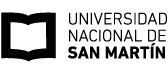
\includegraphics[height=1cm]{./PREAMBLE/logo-unsam.png}
\\} Teoría del funcional de la densidad}
\subtitle[Modelización 2022]{ Modelización de Propiedades y Procesos 2022}
\author{Ruben Weht\inst{1}\inst{2} \and Mariano Forti\inst{1}\inst{3} }
\institute{
  \inst{1}Instituto de Tecnología Prof. Jorge Sabato
  \and
  \inst{2}Fisica del Sólido, Edificio TANDAR, \url{weht@cnea.gov.ar},
  interno 7104
  \and
  \inst{3}División Aleaciones Especiales, Edificio 47 (microscopía),
  \url{mforti@cnea.gov.ar}, interno 7832
}
\subject{DFT}
\keywords{DFT, Density Functional Theory}
\date{2022}

% Inicia el documento.
\begin{document}
% Título de la clase. 
\mode<presentation>{
\begin{frame}[plain]
\titlepage
\end{frame}
}
\mode<article>{
  \maketitle
}
\mode<all>

\section{Introducción}
%\mode<all>
%
%Los cálculos ab initio consisten, a grandes rasgos, en resolver la ecuación de
%Schrödinger para el sistema de electrones e iones particular. Sin embargo, aún para
%sistemas realmente pequeños la cantidad de grados de libertad hace que el sistema se
%vuelva inmanejable.

\mode*
\begin{frame}<presentation>[label=FrameMotivacion]
  \frametitle{Introducción}

  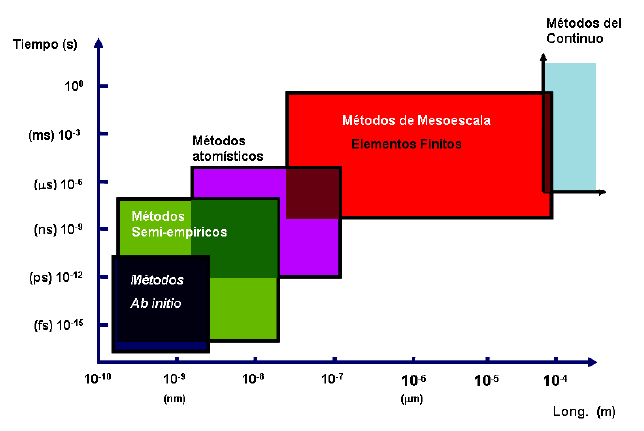
\includegraphics[width=0.5\textwidth]{Figures/Escalas.png}

\end{frame}

%\mode<article>

%Existen estrategias para simplificar el problema. La DFT (Sholl & Steckel 2009; Koch
%& Holthausen 2001) se basa en dos teoremas que Hohenberg y Kohn (HK) enunciaron
%en la decada de 1960 (Hohenberg & Kohn 1964). Estos autores se basan en la idea de
%que en principio toda la información física de la función de onda de un sistema de
%muchos electrones esta contenida en la densidad electrónica. Si $\psi$
% es la función de onda que resuelve la ecuación de Schrödinger del sistema de $N$
% electrones, entonces la densidad electrónica puede definirse como


\mode*
\begin{frame}<presentation>[label=FrameTeorema1]
 \frametitle{Aproximaciones y Teoremas de Hohenverg y Kohn}

 \begin{itemize}

   \item Los núcleos atómicos son suficientemente pesados como para poder considerarlos un potencial externo fijo respecto del sistema electrónico.
     (Born-Oppenheimer)

   \item Toda la información física se encuentra en la densidad electrónica.

   \item La energía del sistema es una funcional de la densidad electrónica.

     $$ E = E[\rho] $$

   \item La densidad electrónica real del sistema minimiza su energía, dado el potencial externo.

     $$ E[\rho_0 + \delta \rho ] \ge E[\rho_0]$$

 \end{itemize}

\end{frame}

\mode<all>

\section{Teoría del funcional de la Densidad}

\newcommand{\eqa}{
  $ \left ( \nabla^2 + V_{Ne}[\rho] +V_{ee}[\rho] +V_{XC}[\rho] \right ) \varphi _\mu = \varepsilon _{\mu} \varphi_{\mu} $
}
\newcommand{\eqb}{
$ \rho_0 (\vec{r}) = \sum _{\mu} f_{\mu} | \varphi | ^2 $
}
\newcommand{\toten}{
  $  E = T [\rho_0] + \int \left ( V_{Ne}+V_{ee} + V_{XC}{\tikz[remember picture, overlay]\node (nxc) at  (-5pt, -5pt) { };} \right ) \rho _0 d \vec{r}  $
}
\newcommand{\eqgga}{
  $  V_{XC} = f \left ( \rho_{\uparrow}, \rho_{\downarrow} , \nabla \rho \right )$
}

\begin{frame}<presentation>[label=FrameSketch]
  \frametitle{Ecuación de Schrödinger vs DFT}
  \begin{columns}
    \column{0.5\textwidth}
      \centering
      \scriptsize
      \texttt{Schrödinger equation}
      \includegraphics[width=\textwidth]{Figures/SketchSchrodingerEq.pdf}
    \column{0.5\textwidth}
      \scriptsize
      \texttt{DFT}

      \includegraphics[width=\textwidth]{Figures/SketchDFT.pdf}
      $$E[\rho] = T[\rho(r)] +V_{ne}[\rho(r)] + V_{ee}[\rho(r)]$$

      E = E\textsubscript{cinética} + E\textsubscript{nucleo-e} + E\textsubscript{electrón - electrón}


  \end{columns}


\end{frame}

\begin{frame}<presentation>[label=KohnShamEquations]

  \frametitle{Kohn - Sham Equations}

    \begin{itemize}

      \item Kohn and Sham Equations , $ \{\varphi\} $ se definen como partículas no interactuantes!

	\vspace{0.5cm}

	\eqa\tikz[remember picture]\node[anchor=center] (A)  {};

	\vspace{0.5cm}


	\eqb\tikz[remember picture]\node[anchor=center] (B)  {};

	\tikz[remember picture, overlay]\path[draw=black, -latex] (B.east) -- ($(B)+(5cm,0)$) |-  (A.east);

      \item Total  Energy

	\toten

	\vspace{1cm}
	\centering \tikz[remember picture]\node (targ) {  GGA-PBE:};

	\eqgga

	\tikz[remember picture, overlay]\draw[black,-latex]   (nxc.south) -- ++(0,-0.1cm) |- (targ.north);

	Potencial de correlación e intercambio: es responsable de modelar los efectos cuánticos. 

    \end{itemize}
\end{frame}


\mode<all>

\begin{frame}<presentation>[label=FrameDFTSolids]

  \centering
  \includegraphics[height=\textheight]{Figures/SketchSolidDFT.pdf}


\end{frame}


\section{Implementación}

\begin{frame}<presentation>[label=FrameSelfConsistantCycle]
  \frametitle{Ciclo Autoconsistente}
  \centering
  \includegraphics[width=\textheight]{Figures/FiguraCicloAutoconsistente.pdf}

\end{frame}



\mode*

\begin{frame}<presentation>[label=FrameBandStructure]
  \frametitle{Cristales}

      Bloch theorem

%	\begin{equation*}
	$$ \varphi_{\mu, k} = \sum_{G} C_{\mu, G, k}  e^{i (\vec{G} + \vec{k} )\cdot \vec{r}} $$  \tikz[remember picture, overlay] \node (A) {};
	%\end{equation*}

	$$ \left ( \nabla^2 + V_{Ne}[\rho] +V_{ee}[\rho] +V_{XC}[\rho] \right ) \varphi _\mu = \varepsilon _{\mu} \varphi_{\mu} $$

Uno termina resolviendo un sistema lineal para cada punto $\vec{r}$ :

    $$ \mathbf{C} _{\mu, \vec {k} + \vec{G} } E[\rho] \varphi _{\mu, \vec{k} + \vec{G}}(\vec {r}) = \varepsilon _{\mu, \vec{k} + \vec{G}} \varphi _{\mu, \vec{k} + \vec{G}}(\vec {r}) $$


\end{frame}

\begin{frame}<presentation>[label=FrameNmerosCunticos]
  \frametitle{Números Cuánticos}
%
$$ \mathbf{C} _{\mu, \vec {k} + \vec{G} } E[\rho] \varphi _{\mu, \vec{k} + \vec{G}}(\vec {r}) = \varepsilon _{\mu, \vec{k} + \vec{G}} \varphi _{\mu, \vec{k} + \vec{G}}(\vec {r}) $$


   \begin{itemize}
      \item $\vec{k} \in BZ $ Red recíproca del sistema ! (por teorema de Bloch). 

      \item $|\vec{k} + \vec{G}| <= K_{max} $ para que la suma sea finita: energía de corte!

      \item $\mu $: niveles de energía o bandas de un cristal

      \item $\varepsilon _{\mu, \vec{k} }$ : estructura de bandas !

    \end{itemize}
%
%
\end{frame}



\end{document}
